\chapter{Introduction}
\label{chap:introduction}

\section{Motivation and Background}
\label{sec:motivation-background}

\subsection{The Machine Learning Context}
Machine Learning (ML) is a branch of Artificial Intelligence that studies algorithms able to learn from data and improve their performance on tasks without being explicitly programmed for every decision rule. Instead of hard-coding each behavior, ML infers a model from observations and then applies that model to prediction, pattern extraction, or decision support.

As the field has matured, a standard taxonomy has emerged. Figure~\ref{fig:ml_taxonomy} summarizes three broad paradigms:
\begin{enumerate}
  \item \textbf{Supervised Learning:} Models learn from labeled input-output pairs to predict future outcomes.
  \item \textbf{Reinforcement Learning:} An agent learns policies through interaction with an environment and reward feedback.
  \item \textbf{Unsupervised Learning:} Algorithms discover patterns, latent structure, or groupings in unlabeled data.
\end{enumerate}

\begin{figure}[H]
  \centering
  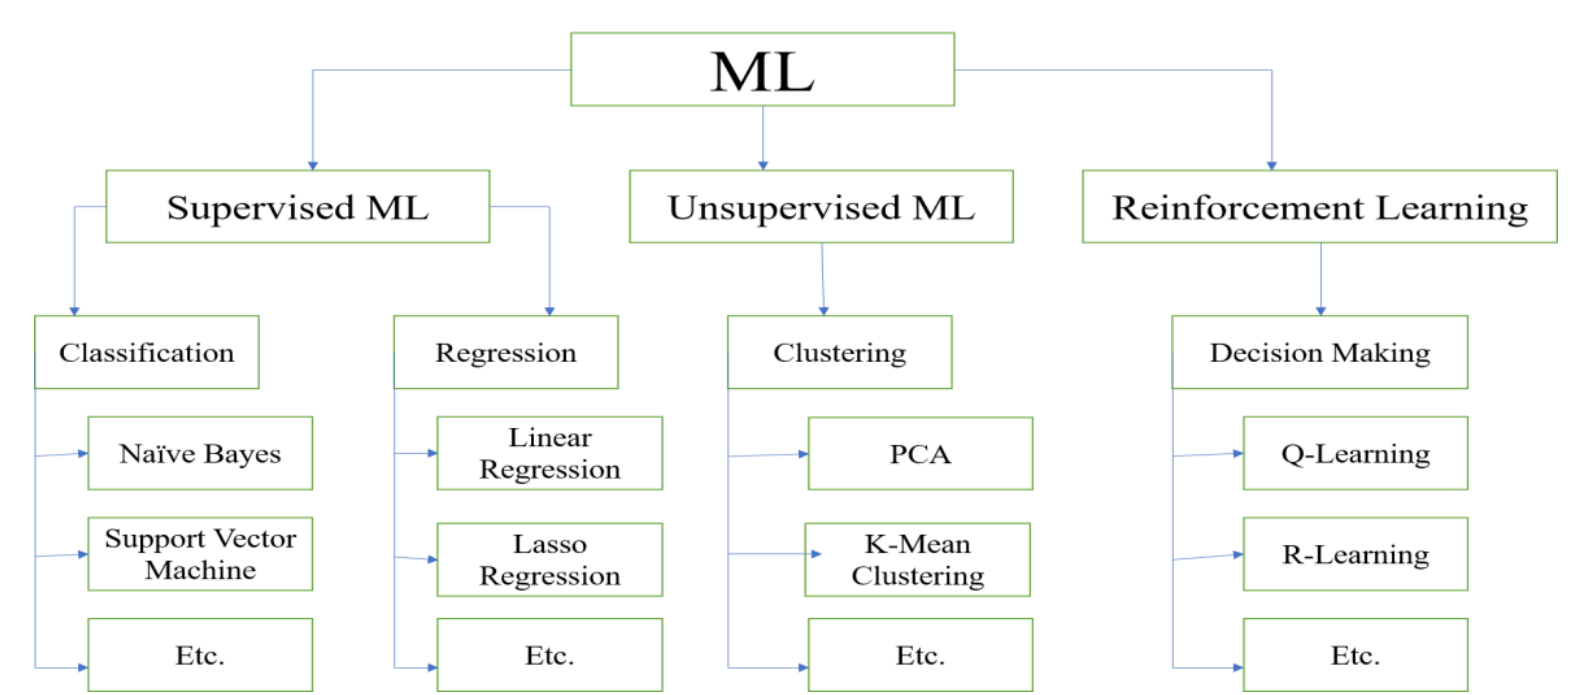
\includegraphics[width=0.85\linewidth]{images/ML_types.png}
  \caption{Taxonomy of common machine-learning paradigms and representative algorithms.}
  \label{fig:ml_taxonomy}
  \source{Compiled by the author}
\end{figure}

\subsection{Clustering in Unsupervised Learning}
This work focuses on clustering, one of the core tasks in unsupervised learning. Unlike supervised methods, clustering algorithms do not observe ground-truth labels during training. Their objective is to infer structure by grouping observations that are geometrically or statistically similar.

Clustering is widely used in exploratory data analysis, customer segmentation, anomaly detection, and scientific discovery. Its performance, however, depends heavily on the geometry of the underlying data. Distances, cluster compactness, density, and distribution shape all affect whether an algorithm can correctly recover the intended partition. Two especially common approaches are:
\begin{itemize}
  \item \textbf{k-means:} A centroid-based algorithm that minimizes within-cluster variance \cite{macqueen1967}.
  \item \textbf{Hierarchical Clustering:} A connectivity-based family of methods that builds a dendrogram of nested partitions \cite{ward1963}.
\end{itemize}

\subsection{The Privacy--Utility Tension}
Although clustering can be highly informative, its application is increasingly constrained by data access. In domains such as healthcare, finance, and public administration, datasets often contain personal or sensitive information and therefore cannot be shared freely for model development or experimentation.

This creates a direct tension:
\begin{itemize}
  \item \textbf{Privacy first:} restricting access protects individuals but limits research and model validation.
  \item \textbf{Utility first:} sharing raw data supports analysis but increases regulatory and ethical risk.
\end{itemize}

\subsection{Synthetic Data as a Candidate Solution}
Synthetic data offers a promising response to this conflict. Instead of publishing real observations, one generates artificial records that preserve the statistical properties, dependencies, and structure of the original dataset while avoiding direct disclosure of real individuals \cite{nowok2016,qian2024}.

In principle, synthetic data should provide both privacy and utility. However, this report evaluates only the utility side of that equation: no explicit privacy-risk experiment is carried out here. The unresolved question is whether the generation process preserves the geometric structures that clustering algorithms depend on. If synthesis distorts cluster boundaries, densities, or relative separations, then downstream clustering quality may collapse even if marginal statistics remain plausible.

\section{Objectives}
\label{sec:objectives}

The primary objective of this report is to evaluate the utility of synthetic data for clustering tasks. More specifically, the study compares K-Means and Agglomerative Hierarchical Clustering on synthetic data generated with the CART method implemented in the \texttt{synthpop} package.

The work is organized around three concrete goals:
\begin{enumerate}
  \item Determine whether clustering algorithms can recover the correct number of clusters from synthetic data as reliably as from the corresponding real data.
  \item Quantify degradation through structural metrics that capture balance, centroid drift, and within-cluster dispersion rather than relying only on cluster-number recovery.
  \item Assess which algorithm is more robust to the geometric distortions introduced by CART-based synthesis, especially in non-normal distributions.
\end{enumerate}

To answer these questions, the project uses a reproducible simulation pipeline with more than 1,800 generated datasets spanning different sample sizes, cluster counts, separations, correlations, and probability distributions. The immediate local antecedent of this report was an earlier exploratory study by Xinnuo Chen, whose name is cited correctly here because that preliminary work motivated the present, more systematic evaluation.

\section{Document Structure}
\label{sec:document-structure}

The remainder of the report follows the seven-chapter structure of the thesis template:
\begin{itemize}
  \item \textbf{Chapter 2} reviews the conceptual foundations of clustering and synthetic data utility, and positions this study against previous work.
  \item \textbf{Chapter 3} formalizes the research questions, experimental requirements, and analytical metrics used to judge utility.
  \item \textbf{Chapter 4} presents the design of the evaluation pipeline, including reference-data generation, synthesis, alignment, and metric computation.
  \item \textbf{Chapter 5} describes the practical implementation choices, toolchain, and reproducibility configuration used in the experiments.
  \item \textbf{Chapter 6} reports the empirical evaluation through PCA, t-SNE, cluster-number recovery, and structural-fidelity measurements.
  \item \textbf{Chapter 7} synthesizes the findings, discusses limitations, and proposes future research directions.
\end{itemize}
